%\input{head.tex}
\subsection{Graphene and hydrogen honeycomb lattice (NE-AIDMD)}
Although only the low energy degrees of freedom are present in the downfolded Hamiltonian, the coefficients of various interacting terms are deeply affected by the high energy degrees of freedom. In other words, the coefficients are renormalized by the high energy degrees of freedom. We demonstrate this renormalization effects from higher energy degree of freedom with an \textit{ab initio} system, graphene. 

Although many electronic properties of graphene can be correctly described in a noninteracting tight-binding model of $\pi$ electrons~\cite{Castro2009}, electron-electron interactions do play a central role in a wide range of phenomena that have been observed in experiments~\cite{Kotov2012}. It is shown that the electron screening from $\sigma$ bonding is very crucial to the correlated physics of graphene, without which graphene would be an insulator instead of a semi-metal \cite{Zheng2016}. Studying the effect of the $\sigma$ electrons on the low energy effective model provides an alternative perspective to understand the screening effect from bonding $\sigma$ electrons. For comparison, we here also study the hydrogen honeycomb lattice with the same lattice constant $a=2.46$\AA, which has similar Dirac cone dispersion as graphene \cite{Zheng2016}. 

 We consider the effective single-band Hubbard model, 
\begin{eqnarray}\label{eq:hubbard}
\hat{H} = C + t\sum_{\langle i,j\rangle}c_{i, \sigma}^\dagger c_{j, \sigma} + \text{h.c.} + U\sum_{i}n_{i, \uparrow}n_{i, \downarrow}\,. 
\end{eqnarray}
The low energy physics is reflected mainly on the dynamics of $\pi$ orbitals in graphene, and $s$ orbitals in hydrogen. Figs.~\ref{fig:wan} (a) and (b) shows the Wannier orbitals of $\pi$ and $s$ orbitals respectively. Due to lack of screening because of zero density of states at Fermi level, the Coulomb interaction is still long range unlike the case in metal where the Coulomb interaction is short ranged because of the formation of electron-hole pairs. However, the effect of the long range part can be considered as a renormalization to the onsite Coulomb interaction $U$ at low energy \cite{Schuler2013, Changlani2015}. Therefore, we expect that Eq.~\eqref{eq:hubbard} is still a relatively good description of the low energy physics. 

\begin{figure*}[hbt]
  \centering  
 % \subfigure[]{\includegraphics[clip, width=0.30\textwidth]{c_sigma.png}}
    \subfigure[]{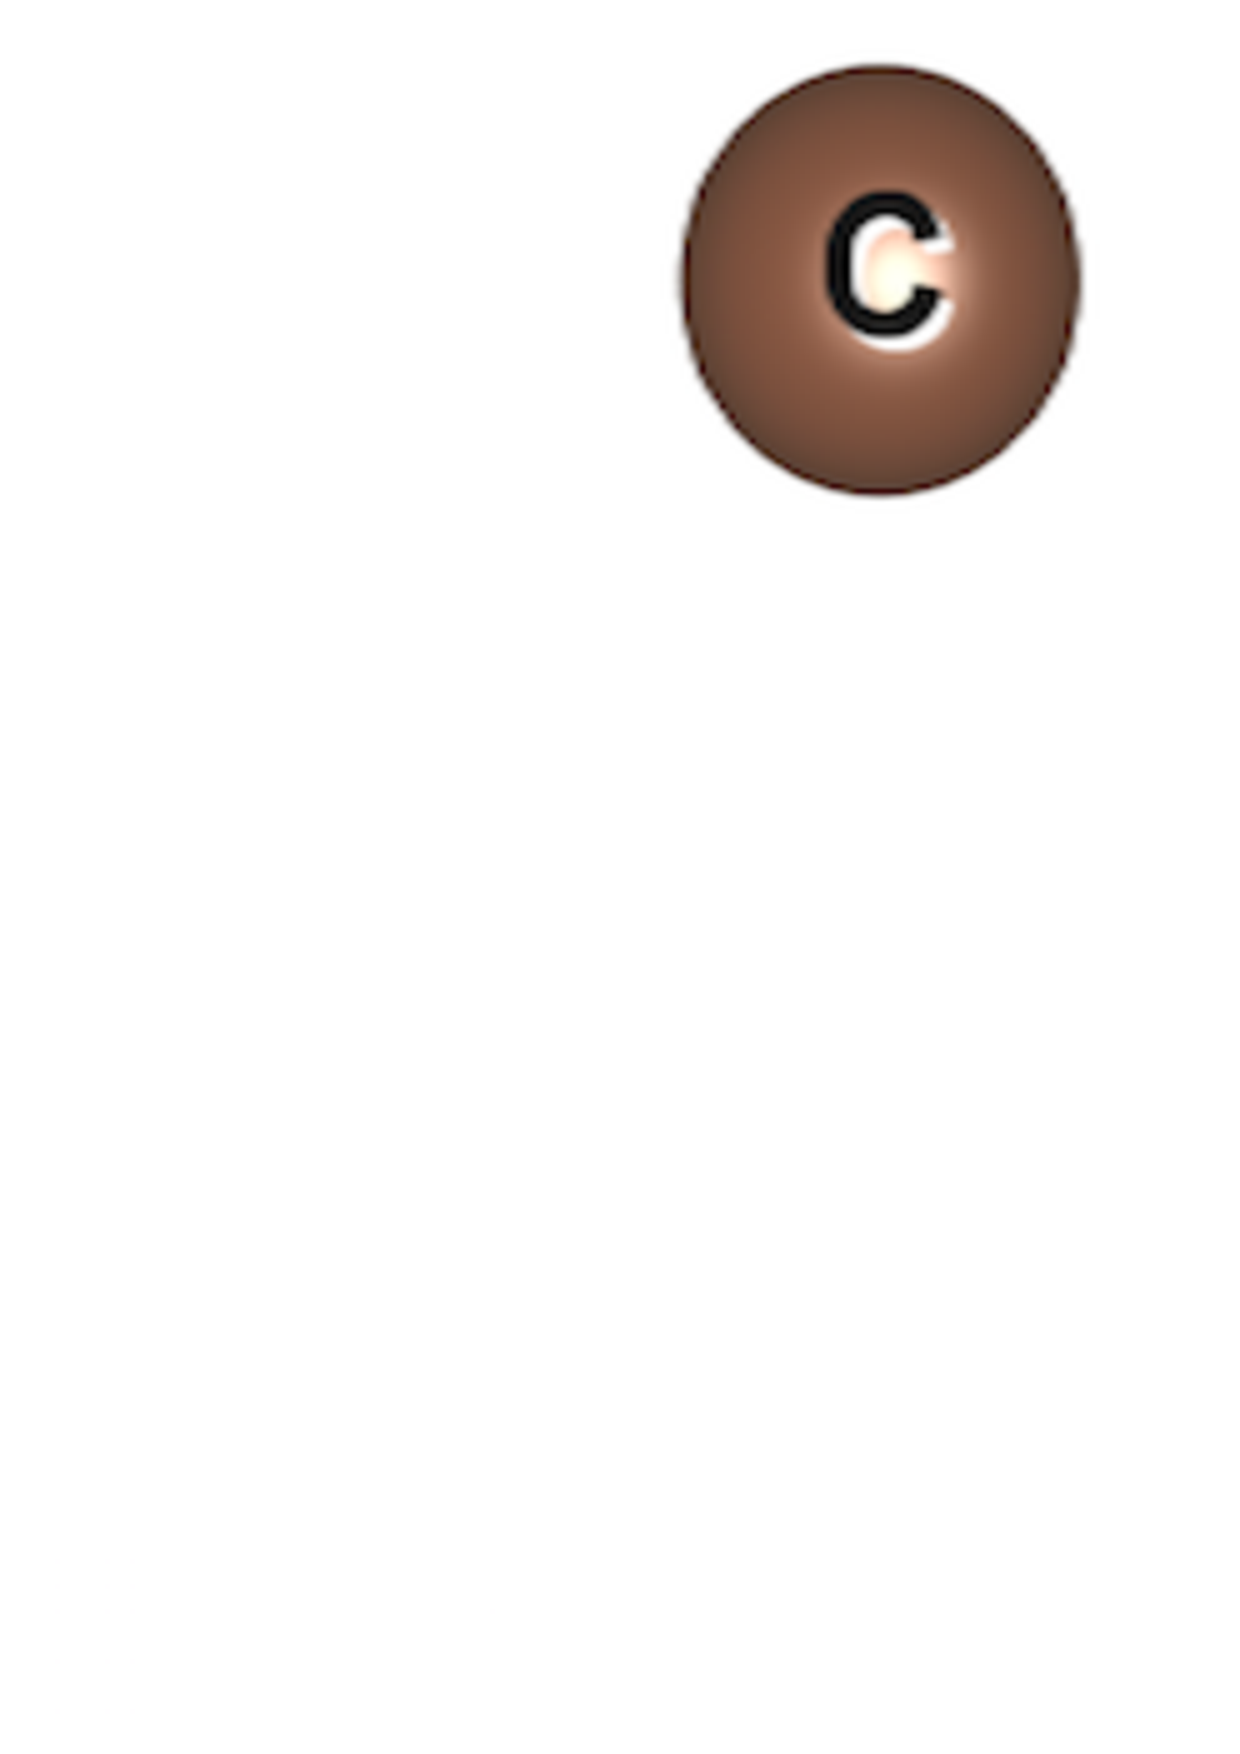
\includegraphics[clip, width=0.30\textwidth]{./Figures/c_pi.png}}
    \subfigure[]{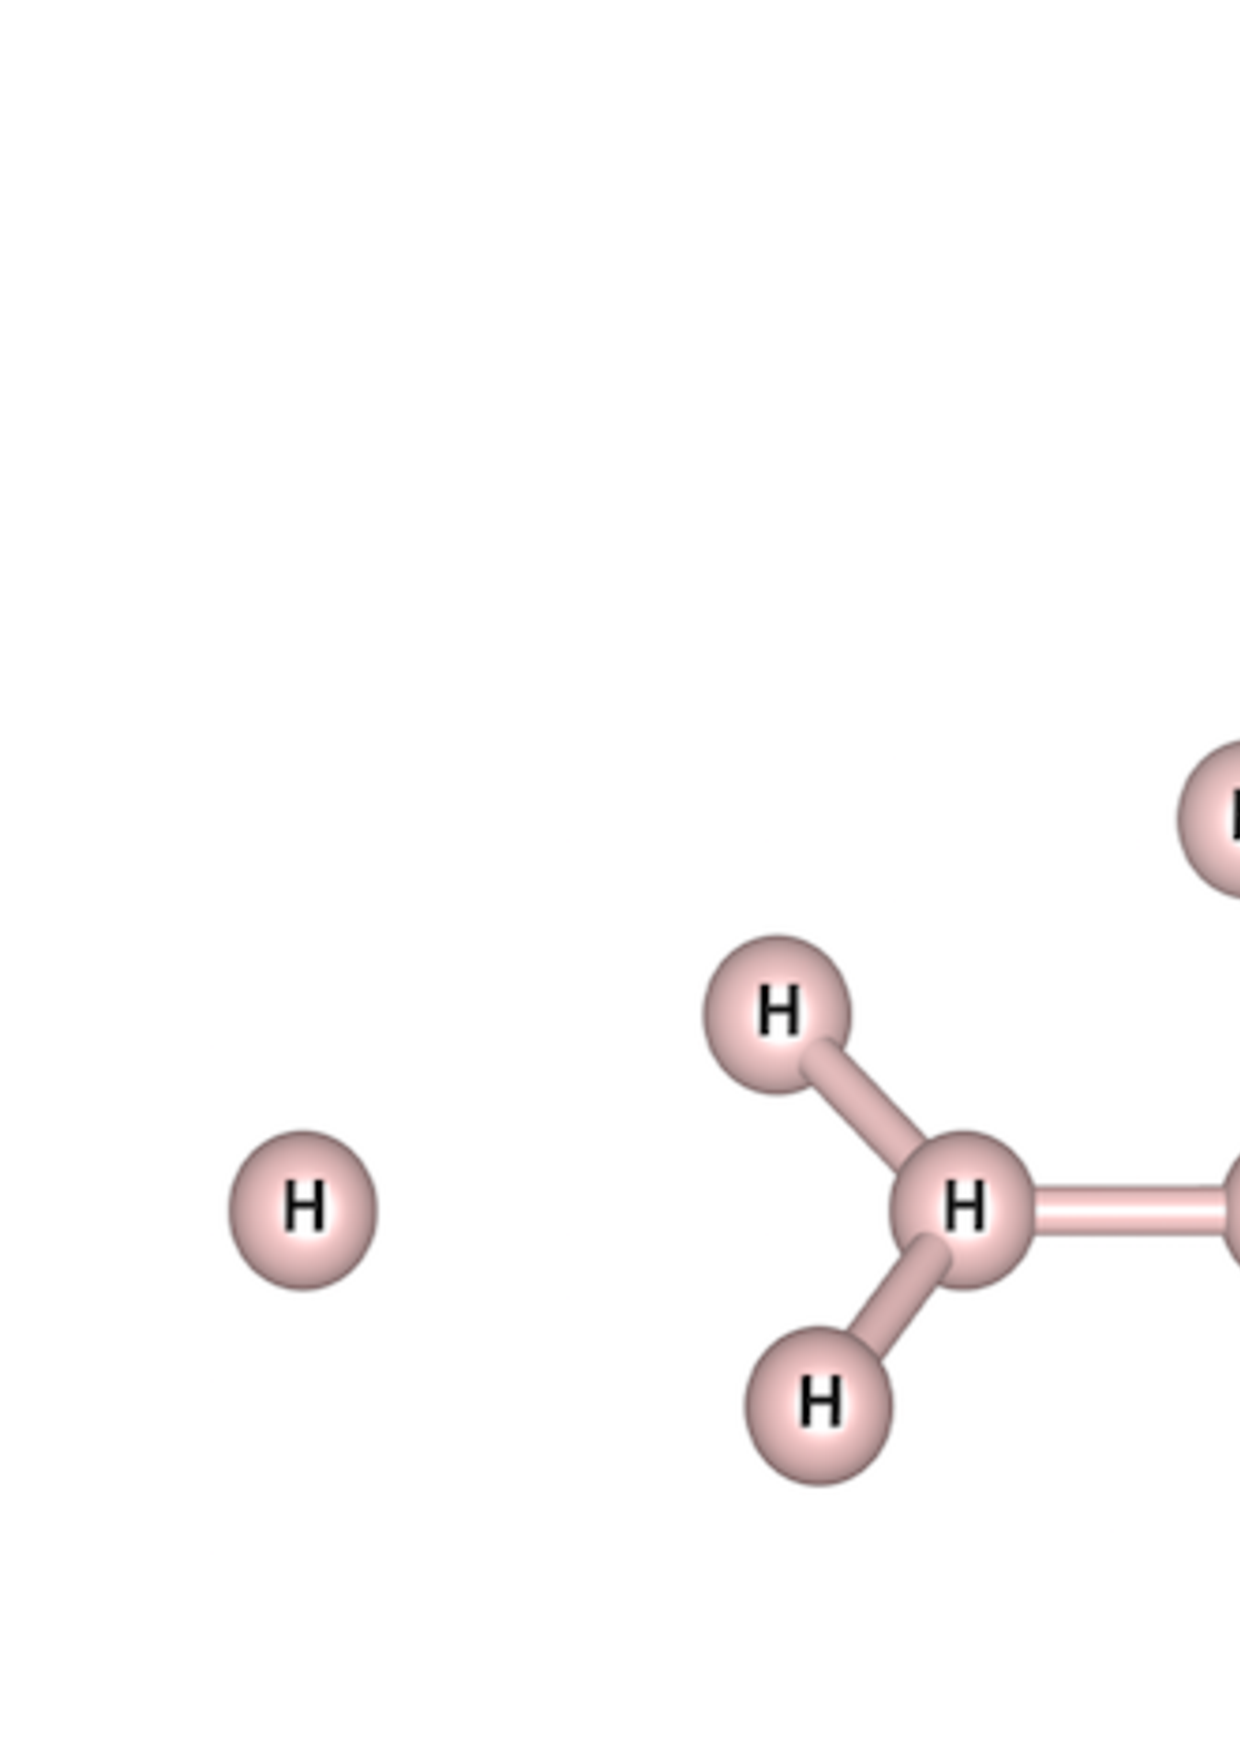
\includegraphics[clip, width=0.30\textwidth]{./Figures/h_wan.png}}
       \caption{Wannier orbitals constructed from Kohn-Sham orbitals: (a) graphene $\pi$ orbitals; (b) hydrogen S orbital. }
\label{fig:wan}
\end{figure*}

We will use the non-eigenstate AIDMD method to obtain the value of $t$ and $U$. We choose a set of Slater-Jastrow wave functions corresponding to the electron-hole excitations within the $\pi$ channel (or $s$ channel for hydrogen system). The energy expectation expressed in terms of the density matrices is, 
\begin{eqnarray}\label{eq:en}
E = C + t\sum_{\langle i, j\rangle, \sigma}( \rho_{ij}^\sigma + \rho_{ji}^\sigma) + U \sum_{i}M_{ii;ii}^{\uparrow,\downarrow}\,.
\end{eqnarray}
where $\rho$ and $M$ are one- and two-body reduce density matrices respectively.

In order to understand the screening effect of $\sigma$ electrons, we also consider a $\pi$-only graphene, in which the $\sigma$ electrons are replaced with a constant negative charge background. The lower energy states we choose for such systems are Slater-Jastrow wave functions constructed from occupied $\pi$ Kohn-Sham orbitals; whereas for the original graphene, the wave functions are Slater-Jastrow constructed from both occupied $\sigma$ bands and occupied $\pi$ bands. 

Table~\ref{tab:grpheffm} shows the final downfolding results of the three systems. The \textit{ab initio} simulations are performed on a $3\times3$ cell. We have used using $25$ low energy states for the downfolding. The error-bar is calculated using Jackniff method. Fig.~\ref{fig:ne_aidmd_gh} shows fitted energies versus the \textit{ab initio} VMC energies. 
\begin{table}[ht]
\label{tab:grpheffm}
\centering
\begin{tabular}{|c|c|c|c|}
\hline
Parameters [eV] & graphene & $\pi$-only graphene &hydrogen \\
\hline
\hline
t & 3.61(1) & 2.99(1) & 3.73(1)\\
U & 7.16(3) & 14.8(2) & 9.47(5)\\
\hline
\end{tabular}
\caption{Downfolding parameters for graphene and hydrogen.}
\end{table} 

We find that the onsite Hubbard model describes graphene and hydrogen very well, as is seen from the small root mean square error of the predicted energies (see Fig.~\ref{fig:ne_aidmd_gh}). The ratio of $U/t$ is small than the semi-metal-insulator transition critical value (3.8) in both graphene and hydrogen, which is consistent to the fact that both the two systems are semi-metals.  The $\pi$-only graphene however has larger $U/t$, and is in the insulating phase. This clearly shows the significance of $\sigma$ electrons in renormalizing the effective onsite interactions of $\pi$ orbitals. Without such screening effect, graphene will be an insulator. This is consistent with previous studies which show that a system of $\pi$ electrons with bare Coulomb interaction will be in insulating phase~\cite{DrutPRL2009, DrutPRB2009,  Smith2014}.
\begin{figure*}[tbh]
\centering
  \begin{tabular}{@{}p{0.95\linewidth}@{\quad}p{\linewidth}@{}}
    \subfigimg[clip, width=0.32\linewidth]{(a)}{./Figures/grp_all_tu.pdf}
     \subfigimg[clip, width=0.32\linewidth]{(b)}{./Figures/grp_pi_tu.pdf}
    \subfigimg[clip, width=0.32\linewidth]{(c)}{./Figures/h_tu.pdf}
      \end{tabular}
\caption{Comparison of \textit{ab initio} (x-axis) and fitted energies (y-axis) of the 3$\times$3 periodic unit cell of graphene and hydrogen lattice: (a) graphene; (b) $\pi$-only graphene; (c) hydrogen lattice.}\label{fig:ne_aidmd_gh}
\end{figure*}

%\input{tail.tex}
